\documentclass[acmtocl,acmnow]{acmtrans2m}
\usepackage{amssymb}
\usepackage{amsmath}
\usepackage[dvips]{epsfig}

\newcommand{\R}{I\!\!R}
\newcommand{\OpenAD}{OpenAD}
\newcommand{\OpenSixtyFour}{Open64}
\newcommand{\OpenAnalysis}{OpenAnalysis}
\newcommand{\OpenADFortTk}{OpenADFortTk}
\newcommand{\XAIF}{XAIF}
\newcommand{\xaifBooster}{xaifBooster}
\newcommand{\whirlToxaif}{whirl2xaif}
\newcommand{\xaifTowhirl}{xaif2whirl}
\newcommand{\reffig}[1]{Figure~\ref{#1}}
\newcommand{\refsec}[1]{Section~\ref{#1}}

\markboth{Lots Of Authors et al.}{\OpenAD}

\title{\OpenAD: A tool for automatic differentiation 
of Fortran90 codes}

\author{PATRICK HEIMBACH, CHRIS HILL, DERYA OZYURT, CARL WUNSCH\\Massachusetts Institute of Technology\\
MIKE FAGAN, NATHAN TALLENT \\Rice University\\
MICHELLE STROUT, JEAN UTKE \\Argonne National Laboratory 
\and
UWE NAUMANN\\Rheinisch Westf\"alische Techinische Hochschule Aachen}

\begin{abstract}
The \OpenAD\ tool allows the evaluation of first and second order 
derivatives of functions defined by a program written in Fortran90/77. 
The derivative evaluation is performed by Fortran 90 code resulting from the 
analyses and transformation of the original program that defines the function of interest.
The code transformation follows the basic principles of automatic differentiation. 
In difference to most other automatic differentiation tools \OpenAD\ is 
built from components that permit an easy extension of the code transformations 
in a language indepdendent fashion. It uses code analysis results implemented 
in the \OpenAnalysis\ component. 
The interface to the language independent transformation 
engine is an xml abstract interface format, called \XAIF\ that is  specified through an xml schema. 
The implemented transformation algorithms allow efficient derivative computations utilizing 
locally optimized cross country  sequences of vertex, edge and face elimination steps. 
Specifically for the generation of adjoint codes \OpenAD\ supports various code reversal 
schemes with hierachical checkpointing at the subroutine level. 
The Fortran specifive front and back end to this transformation engine is the \OpenSixtyFour\ based
\OpenAD\ Fortran tool kit, \OpenADFortTk.
\end{abstract}


\category{G.1.4}{Quadrature and Numerical Differentiation}{Automatic differentiation}
\category{D.3.4}{Processors}{Code generation, Compilers}
\category{F.3.2}{Semantics of Programming Languages}{Program analysis}
\category{G.1.6}{Optimization}{Gradient methods}

\terms{Algorithms, Performance}

\keywords{Automatic differentiation,  source transformation, adjoint compiler}

\begin{document}


\begin{bottomstuff} 
P.~Heimbach, C.~Hill, D.~Ozyurt, and C.~Wunsch, Massachusetts Institute of Technology, 
Boston, MA XXXXX;\newline
M.~Fagan, N.~Tallent, Rice University, 
Houston, TX XXXXX;\newline
M.~Strout, J.~Utke, Argonne National Laboratory, 
Argonne, IL XXXXX;\newline
U.~Naumann, Rheinisch Westf\"alische Techinische Hochschule Aachen, 
D-XXXXX Aachen, Germany;\newline
Funding for the ACTS project is provided by NSF under ITR contract OCE-0205590
for a three year period that started in September 2002.
\end{bottomstuff}
\maketitle

%#########################################################################################
\section{Introduction} \label{sec:Introduction}

The basic principles of automatic differentiation (AD), see also \refsec{ssec:ADmath}, 
have been known for several decades \cite{wengert}
but only during the last 15 years the tools implementing AD have found a noticable use in 
optimization, data assimilation, and other applications in need of efficient and accurate 
derivative information. 
As a consequence of the wider use of AD 
a variety of tools have been developed that address specific 
application requirements or programming languages. 
The website {\tt www.autodiff.org} provides a good overview of the tools that 
are currently available. 
One may characterize two user groups of AD tools. On one side are the casual users 
with small scale problems applying AD mostly in a black box fashion and demanding 
minimal user intervention. 
On the other side are experienced AD users aiming for highly efficient 
derivative computations. Their need for efficiency is dictated by the 
computational complexity of models that easily reaches the limits of  current 
supercomputers. With the emphasis on efficiency some sacrifices on the support of 
language features are acceptable for this user group. 

One of the most demanding applications of AD is the computation of gradients for 
data assimilation on large scale models used in oceanography and climate research. 
An evaluation of the available tools revealed some shortcomings from the perspectives 
of the tool users as well as the tool developers. 

From  the AD tool  users point of view ... FILL IN

From the AD tool developers point of view ... FILL IN

These issues became the motivation for the 
Adjoint Compiler Technology \& Standards (ACTS) project\footnote{ 
see {\tt www.stce.rwth-aachen.de/ACTS}
}. 
This project is a collaborative
research and development effort between MIT, Argonne National Laboratory, 
Univeristy of Chicago, and Rice University. 
It focusses on  next-generation tool development and 
application of AD to problems in oceanography and chemical engineering.
The main result of this effort is an infrastructure for the language independent 
development and use of AD algorithms. 
\OpenAD\ is the Fotran90 incarnation of the infrastructure.\footnote{
The C/C++ oriented ADIC version 2.0 is based on the same infrastructure and can be found
at {\tt www.mcs.anl.gov/adicserver}.
}
\begin{figure}[htb]
\centerline{ 
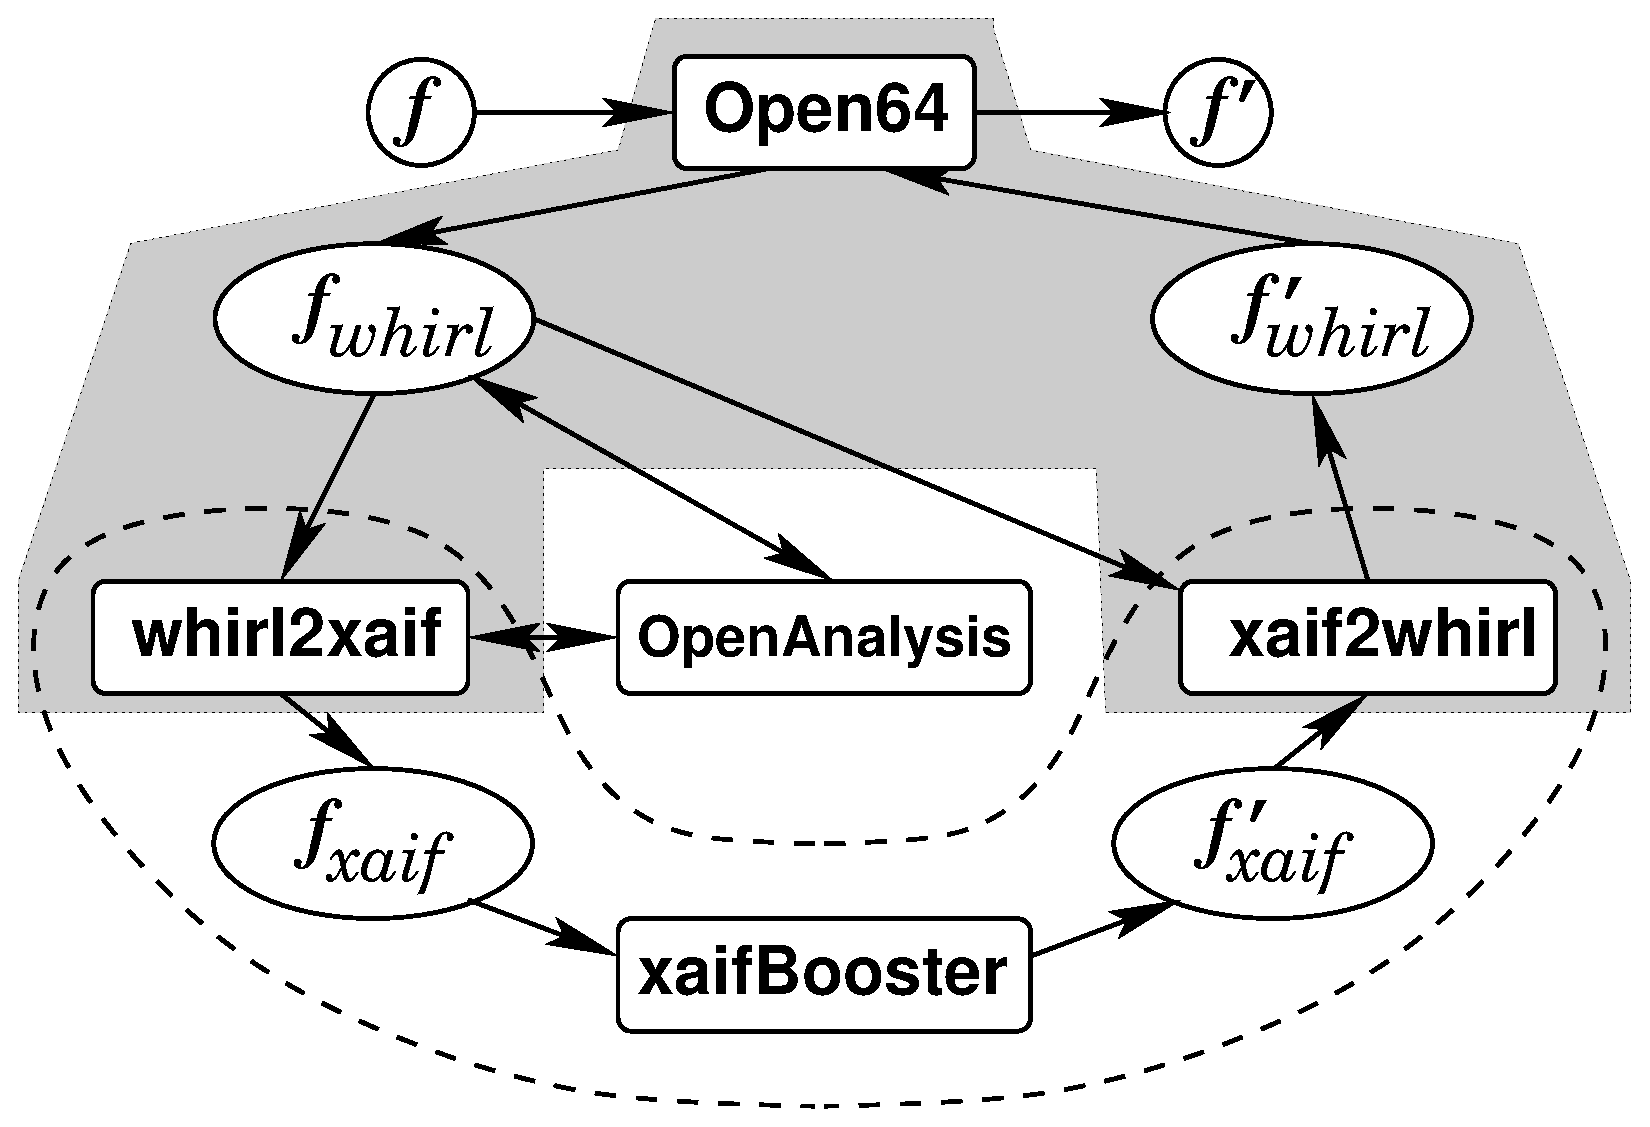
\epsfig{file=overview.eps,width=6cm}
}
\caption{\OpenAD\ components and pipeline} \label{fig:overview}
\end{figure}
The collaboration  of the \OpenAD\  components is illustrated in 
\reffig{fig:overview}
The \OpenSixtyFour\ front-end performs a lexical, 
syntactic, and semantic analysis and produces an 
intermediate representation of $F$ in the so-called {\em whirl} format.
\OpenAnalysis\ is used to build call and control flow graphs and  perform 
code analyses such as alias, activity, side-effect analysis.
This information is used by 
\whirlToxaif\ to construct a representation of the numerical core of $F$ in
\XAIF\ format shown as $F_{xaif}$.  
A differentiated version of $F_{xaif}$ is derived by an 
algorithm that is implented in \xaifBooster\ and is again respresented 
\XAIF\ as $F'_{xaif}$.
The information in $F'_{xaif}$ and the original $F_{whirl}$ are used by 
\xaifTowhirl\ to construct a 
{\em whirl} representation $F'_{whirl}$ of the differentiated code. 
The unparser of 
\OpenSixtyFour\ transforms $F'_{whirl}$ into Fortran90, thus completing
the semantic transformation of a program $F$ into
a differentiated program $F'$.
The dotted line encloses the language specific front-end that can potentially
be replaced by front-ends for languages other than Fortran. 
For example, an 
effort running parallel to the ACTS project at Argonne National Laboratory is 
developing a new version of ADIC \cite{HoNo01} by coupling a C/C++ 
front-end 
based on an EDG parser ({\tt www.edg.com}) and uses ROSE in combination with SAGE~3 ({\tt www.llnl.gov/CASC}) as internal representation
with \OpenAD.

This paper discusses the components of \OpenAD,
including the underlying design decisions, algorithmic aspects, and
numerical results.
 





\subsection{Formal description of Automatic Differentiation}

In this section we introduce the notational framework we will refer to throughout 
this paper. A detailled introduction to AD can be found in \cite{Gri00}. 
We would also like to refer the reader to the proceedings of four conferences 
on AD \cite{CG91,BBCG96,CFG+01,BCH+05}.







%#########################################################################################
\section{\OpenAD\ components}
%-----------------------------------------------------------------------------------------
\subsection{xaif} 
An XML-based ({\tt www.w3c.org/XML}) hierarchy of directed graphs, referred to as xaif 
\cite{HNN02}, is used for the 
internal representation of the numerical core of the implementation
of a given vector function. This format is 
well suited to represent the results of  semantic transformations including 
preaccumulation \cite{BiHa96,CDB96,GrRe91} and 
program reversal \cite{Gri92,WaGr01} at various levels (call graph, control 
flow graphs, basic blocks, expressions). 
The main idea behind xaif is to provide a language-independent exchange
format that separates language-specific from transformation-related 
algorithmic issues. Potentially, front-ends for various programming languages 
can utilize xaif, for example, \OpenSixtyFour\ and EDG/SAGE~3 as pointed out before.

%-----------------------------------------------------------------------------------------
\subsection{\xaifBooster} 
\begin{figure}
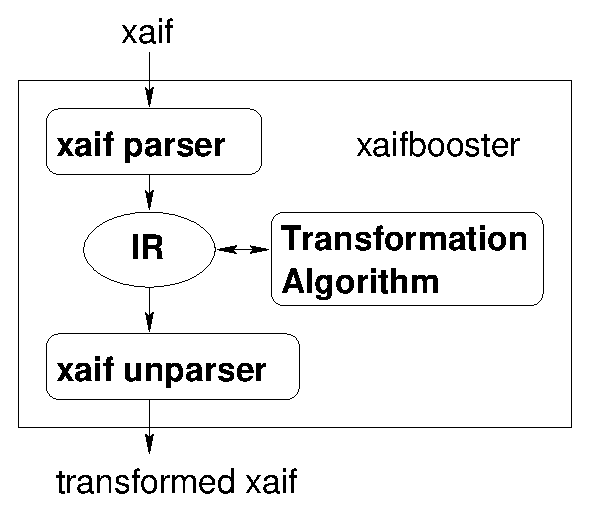
\epsfig{file=principle.eps,width=4cm}
\caption{\xaifBooster\ parses xaif code into an internal representation (IR).
It provides an API for transformation algorithms to modify the IR. An unparser
returns the transformed xaif code.} \label{fig:xaifBooster}
\end{figure}
The C++ code \xaifBooster\ is a collection of utilities and routines for the
(semantic) transformation of programs given in xaif. Its principal architecture 
is illustrated in \reffig{fig:xaifBooster}. One of the major concerns during
the development of \xaifBooster\ has been the clean separation of the internal
representation (an enhanced object image of xaif) from algorithms that operate 
on this data structure. This goal has been achieved by applying the design 
patterns \cite{DesignPatterns} factory, visitor, and decorator as described in \cite{UtNa03}.
The result is an API that gives AD developers the opportunity
to implement new algorithms in a source transformation environment without
having to implement full compiler front- and back-ends. Building on
this API, we have implemented a tangent-linear algorithm that uses statement-
\cite{SEUpreacc} and basic-block-level preaccumulation of local 
gradients/Jacobians. Near-optimal face elimination \cite{ElimTechMP} sequences 
are computed by the software tool 
ANGEL \cite{AGN03,SAGA} ({\tt angellib.sourceforge.net}) and transformed into 
Jacobian code by
an \xaifBooster\ algorithm. A simple adjoint version of the code is obtained
by taping the local Jacobians 
and by computing the corresponding ``transposed Jacobian-vector" products 
during an interpretive reverse sweep through the tape. This approach is
essentially equivalent to split program reversal \cite{Gri00} and allows
for an easy coupling of tangent-linear and adjoint versions of small to 
medium-sized codes as described in \cite{NaHe03}. 

Details of the automatic generation of adjoint code in split mode are presented
in the full version of the paper. Furthermore, additional information is 
provided on \xaifBooster\ as a platform for implementing new AD algorithms with 
the objective to establish an open quasi-standard development infrastructure
within the AD community.
%-----------------------------------------------------------------------------------------
\subsection{Fortran~90 front-end} 
The main target application of the ACTS project is the MIT general circulation
model (MITgcm) \cite{mars-eta:97b,mars-eta:97a}. 
It is mostly implemented in Fortran~77 to permit maintenance of an efficient
and correct adjoint as the code evolves \cite{HHG02}. Future development will
increasingly add Fortran~90 features. We use the Fortran~90 
front-end that is part of the \OpenSixtyFour\ compiler suite 
maintained by the Center for High Performance Software
Research at Rice University 
({\tt hipersoft.cs.rice.edu/OpenSixtyFour/}). It parses
Fortran codes into an intermediate representation called whirl and
provides an unparser from whirl back to Fortran. 
The focus of the ACTS project is on the
transformation of whirl into xaif (\whirlToxaif) and, conversely, on the
back-translation of differentiated xaif code into whirl (\xaifTowhirl). 
\whirlToxaif\ uses the call graph and control flow graph builders that are part 
of the \OpenAnalysis\footnote{No documentation is available yet. 
Refer to the \OpenSixtyFour\ cvs repository under 
{\tt hipersoft.cs.rice.edu/Open64} for information on the code.} 
infrastructure, whose objective is to provide a programming
language-independent platform for the development of data and control flow 
analyses. 
%-----------------------------------------------------------------------------------------
\subsection{\OpenAnalysis} 

%#########################################################################################
\section{Application}

The reference application for the first prototype of an \OpenAD\ implementation
is a simplified oceanographic box model for investigating
thermohaline circulation. It relates to the
ocean circulation's role in the variability of the climate system,
on time scales of decades to millennia \cite{tzi-ioa:02}.
Previously, the AD tool TAF \cite{GiKa02} 
had been used to generate the derivative
code in both forward and reverse modes.
See \cite{maro-eta:99} for an applications of
TAF's predecessor TAMC to the MITgcm.

\OpenAD\ has been used to generate tangent-linear and 
adjoint versions of the box model. We established numerical identity between
the Jacobians provided by TAF and \OpenAD.
The successful 
application of \OpenAD\ to the box model code is considered as a feasibility 
proof for the overall approach taken by the ACTS project.  
%-----------------------------------------------------------------------------------------
\subsection{Shallow Water Model}
%-----------------------------------------------------------------------------------------
\subsection{Derya's application}

%#########################################################################################
\section*{Ongoing Work: Reverse Mode}

Ongoing efforts target the automatic generation of efficient adjoint
code by using the reverse mode of AD. Checkpointing is realized at the 
subroutine level allowing for the storage of inputs as well as outputs. 
For each subroutine we generate a version that ``knows" how to store and 
restore its arguments and results, how to run (parts of) itself for a given
set of inputs, and how to tape and immediately adjoin (parts of) itself.
This approach allows for a large number of reversal modes, 
joint mode \cite{Gri00}, and joint mode with subroutine results checkpointing 
representing special cases. 

We expect to have a first version of the reverse mode with checkpointing
running by the end of April. The full paper describes the approach in detail 
and presents numerical results.

%#########################################################################################
\section*{Conclusion and Future Work}

\OpenAD\ is an AD tool development infrastructure. Its well-separated components
allow developers to focus on various aspects of source-to-source 
transformation AD, including parsing and unparsing of different programming
languages, data and control flow analysis, and (semantic) transformation 
algorithms. The intention of \OpenAD\ is to provide the AD community with 
an open, extensible, and easy-to-use platform for research and development
in the field. Its intention is not to render obsolete existing source transformation
tools such as ADIFOR,\footnote{{\tt http://www.cs.rice.edu/\~\!adifor}} 
the differentiation-enabled NAG Fortran 95 
compiler,\footnote{{\tt http://www.nag.co.uk/nagware/research/ad\_overview.asp}} TAF,\footnote{{\tt http://www.FastOpt.de}} and TAPENADE.\footnote{{\tt http://tapenade.inria.fr:8080/tapenade/index.jsp}} 
Their closer coupling with the language-specific internal representation of 
the program has the potential to make the
exploitation of certain language features easier. \OpenAD\ is supposed to 
complement these tools by providing well-defined APIs to an open internal 
representation that can be used by a large number of AD developers.
Users of AD technology will benefit from the expected wide
variety of combinations of front-ends and algorithms that is made possible
by \OpenAD.

During the remainder of the ACTS project we will focus on the implementation
of robust and efficient data flow algorithms in \OpenAnalysis, including alias, 
define-use and use-define, in-out \cite{Muc97}, 
activity, and to-be-recorded \cite{HNP02} as well as on 
the development of various reverse mode algorithms for parallel MPI codes
combining elements such as preaccumulation and (automatic) checkpointing
\cite{Gri92}. 
A second set of target 
applications in chemical engineering \cite{FTB97} requires combinations of first and 
second derivatives in addition to methods for exploiting structure and sparsity
of the underlying computation. We intend to investigate ways to compute these
combinations efficiently by integrating \OpenAD\ into the relevant 
numerical algorithms.

Ultimately, our aim is to generate correct, efficient, scalable, and easily 
maintainable adjoint code for the MITgcm. The major challenge arises from the
requirement to tackle problems in which derivatives are calculated with respect 
to billions of controls. A combination of the methods outlined above is 
essential to guarantee the successful completion of this highly ambitious
project.


\bibliographystyle{acmtrans}
\bibliography{openad}


\begin{received}
Received May 2005;
\end{received}

\end{document}
